\section{Algoritmo di selezione della domanda}
Le domande che verranno presentate durante un allenamento verranno scelte secondo lo \textit{skill level} dell'utente. L'algoritmo funzionerà come segue:
\begin{enumerate}
	\item Verifica lo \textit{skill level} dell'utente;
	\item Definisce il range di possibili domande da presentare all'utente;
	\item Genera uno o due numeri casuali compresi tra 1 e 100 che permettono di scegliere in quale intervallo di probabilità pescare la domanda, secondo i valori indicati in tabella.\\
Generazione del primo numero:
	
	%TABELLA
\begin{center}
\scalebox{0.88}{
\begin{tabular}{|c|c|}
	\hline
	Numero generato & Range della domanda \\ \hline
	1 - 50 & 580 - 620 \\ \hline
	51 - 75 & 621 - 660 \\ \hline
	76 - 85 & 661 - 700 \\ \hline
	86 - 95 & 540 - 579 \\ \hline
	96 - 100 & 500 -539 \\
	\hline
\end{tabular}
}
\end{center}

Nel caso in cui il primo numero generato sia compreso tra 1 e 50, l'algoritmo ne genera un secondo:

	%TABELLA
\begin{center}
\scalebox{0.88}{
\begin{tabular}{|c|c|}
	\hline
	Numero generato & Range della domanda \\ \hline
	1 - 70 & 600 - 620 \\ \hline
	71 - 100 & 580 - 599 \\
	\hline
\end{tabular}
}
\end{center}

	\item Sceglie una domanda casuale da questo insieme.
\end{enumerate}
Qui di seguito proponiamo un'immagine rappresentativa di come funziona l'algoritmo per facilitare la comprensione.

% IMMAGINE RAPPRESENTATIVA
\begin{figure}[ht]
	\centering
	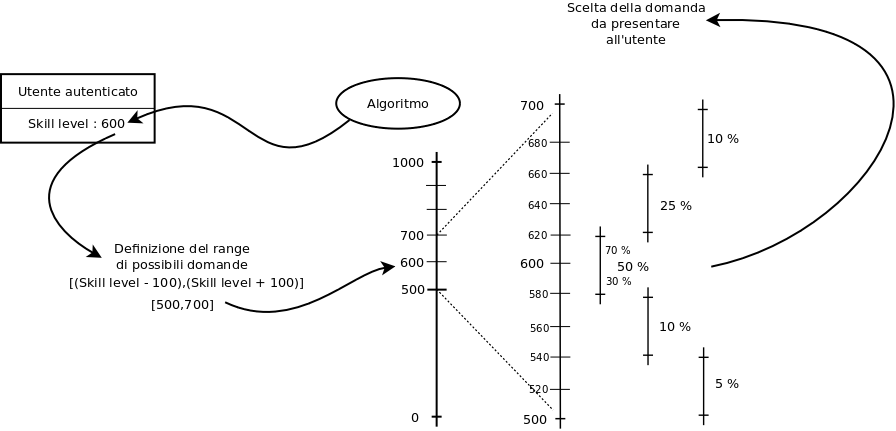
\includegraphics[scale=0.30]{UML/algoritmo.png}
	\caption{Funzionamento Algoritmo di selezione della domanda}
\end{figure}
\FloatBarrier
